\chapter{Methodologies}
\graphicspath{{Chapter3/Figs/}{Chapter3/Figs/}}

This chapter describes the project-related academic methodologies in the given context of the author and the planned approach to achieve the thesis's goals and objectives. The reader is introduced to the rationale for the intended workflows, hardware, and software tools.

\section{Derivation of the case study}
\label{chapter3-derivation-of-the-case-study}

In October 2021, the author began working as a cloud software engineer at IDUN Technologies, an ETH-spin-off startup located in Zürich, to further develop existing software products. IDUN Technologies had already created a PoC software system that included a web-based single-page application (SPA) hosted on AWS Amplify, a backend-as-a-service aiming to simplify the deployment of backends for mobile or web apps. IDUN's in-ear headphone sensor sent EEG data to a network bridge via Bluetooth and then to the cloud via the internet. The raw EEG data was saved and available for download in various file formats.

\begin{figure}[!ht]
  \centering
  
\includegraphics[width=\linewidth]{raw-filtered-data.png}
  \caption{Difference between raw and filtered EEG data from IDUN's in-ear device.}
  \label{fig:raw-filtered-eeg}
\end{figure}

In addition to raw data, the IDUN SPA provided transformed data, such as, e.g. filtered data, which included low-pass and high-pass filtering of EEG data as shown on \autoref{fig:raw-filtered-eeg}. This transformed EEG data was then saved alongside the raw version on the cloud.

The EEG data could also be visualised in near-real-time on the SPA as a time-series x- and y-axis plot. Additionally, users could control the device by sending start and stop commands to the hardware components. The architecture overview is displayed on \autoref{fig:idun-amplify} in which IDUN GDK refers to the IDUN Guardian Development Kit.

\begin{figure}[!ht]
  \centering
  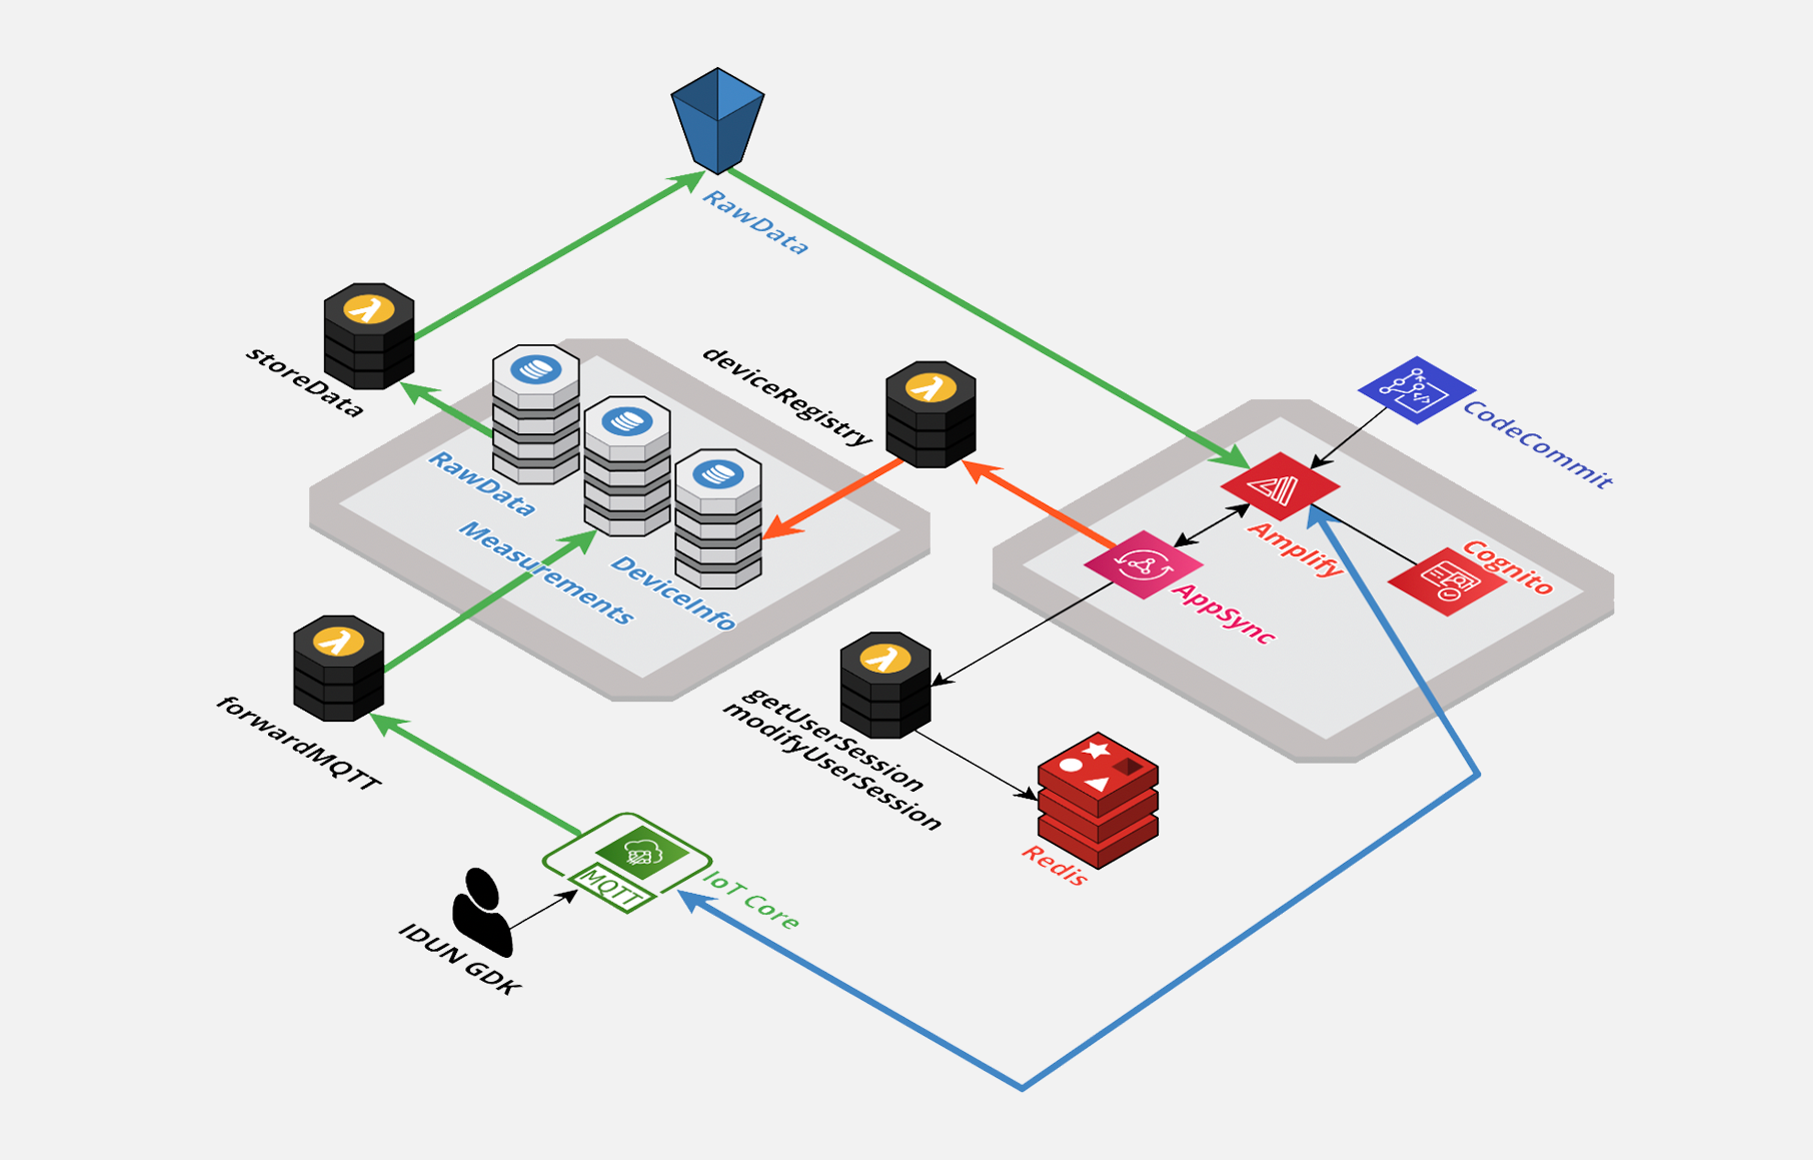
\includegraphics[width=\linewidth]{idun-amplify.png}
  \caption{IDUN's software architecture at the end of 2021.}
  \label{fig:idun-amplify}
\end{figure}

The system was in a relatively unstable state and had strange error sources that made it impossible to reliably record EEG data for more than a few minutes, making the product unusable for existing customers or a mass-market launch. While working on the system, the author encountered various amount of technological flaws and problems as listed in the following list:

\begin{itemize}

\item AWS Amplify is great for frontend developers who want to build simple backends with CRUD\footnote{CRUD is an acronym describing general operations of a backend system: Create, Read, Update and Delete.} operations, but it is not intended for anything custom-made, such as e.g. the streaming-focused aspect of EEG data. Therefore, AWS Amplify must be abandoned as soon as possible, or the project will be built with the wrong tools and foundations.
\item The network bridge was a Raspberry Pi 4 Model B running Python code, which after some analysis, turned out to be the primary source of most of the bugs due to limits in computational power. The question was raised whether the network bridge was needed since IDUN intends to build a completely mobile system, not tied to a network and directly connected to e.g. a mobile phone.
\item The cloud's heartbeat functionality was missing, which meant that the cloud knew nothing about the hardware devices, and simply assumed that data would flow in as soon as the start command was sent to the device, creating a pure happy path scenario.
\item The cloud infrastructure was automatically provisioned by AWS Amplify, which uses AWS CloudFormation as its core, which is an infrastructure as code (IaC) tool, that was run inside of AWS CodePipeline, AWS' continuous integration service, which made everything coupled to specific AWS services where the technical decision to use them was not made based on reasoning but based on the Amplify's creators to use them.
\item All software in the cloud was built using the AWS Console (the AWS GUI). Therefore, no current state in the form of IaC reflected the current infrastructure, which made it impossible to reproduce the cloud in different environments, e.g. prevent blast radius' if something went wrong.
\item The data was streamed via IBM MQ Telemetry Transport (MQTT), a publish-and-subscribe transport protocol commonly used for IoT devices that e.g. regularly send telemetry data. The purpose of MQTT was not to send high-frequency EEG data in real-time but to minimise network bandwidth. Therefore, there was also a need to rethink this technological decision based on the nature of IDUN's EEG sensor, which produces 250 EEG samples per second.
\item The SPA was a thick client, meaning that it ran a lot of business logic, such as filtering raw data for real-time visualisation, which was another technological misstep, as the client-side JavaScript ecosystem is far inferior compared to, e.g. the Python ecosystem that could run in the backend to handle such tasks. If possible, shipping business logic that could hold intellectual property to clients should be avoided if possible, especially with a commercial product.
\item The SPA was not connected to a single endpoint on the backend and used the MQTT stream and the non-real-time aspects of the app (e.g. login or list of recorded EEG data) via different sources. For example, the MQTT stream was subscribed directly from the device itself and did not run through AWS Amplify's GraphQL API, which made coupling the systems into a coherent and robust API cumbersome.
\item The state of the whole application was difficult to handle due to the decoupled logic from the streaming aspect and non-real-time GraphQL API. Combined with the lack of a hardware heartbeat, it was very tedious to figure out what the user was doing and what was being sent. As an interim solution, AWS ElastiCache, a provisioned service for in-memory databases like Redis, was set up, but the state was traded in the SPA and on ElastiCache at the same time. For example, if a user closed the browser tab during a data stream, the stream was stopped, and the EEG data was sent to the void.
\end{itemize}

Due to growing problems with the existing software system and an ever-increasing technical debt as a result of the software not being test-driven or developed without code quality standards, resulting in bugs and quirks that are difficult to track down, the author proposed to halt the implementation of new features and restructure the system from the ground up using a more software engineering-oriented approach. The company's management approved the request for such risky redevelopment in early December of 2021. At the time the author was already working on his original Bachelor project, which focused on a mind-controlled multiplayer game, assuming that IDUN's software system would be stable by the time the Bachelor project began. The original bachelor project's focus was officially changed at the end of 2021 to create a thesis on this refactored software system.

\section{Case study}
\label{chapter3-case-study}

As mentioned in previous chapters, IDUN manufactures an EEG sensor in the form of in-ear headphones. Their vision is to sell their hardware and license a software product coupled with the hardware called Neuro-Intelligence Platform (NIP), as shown on \autoref{fig:idun-nip}.

\begin{figure}[!ht]
  \centering
  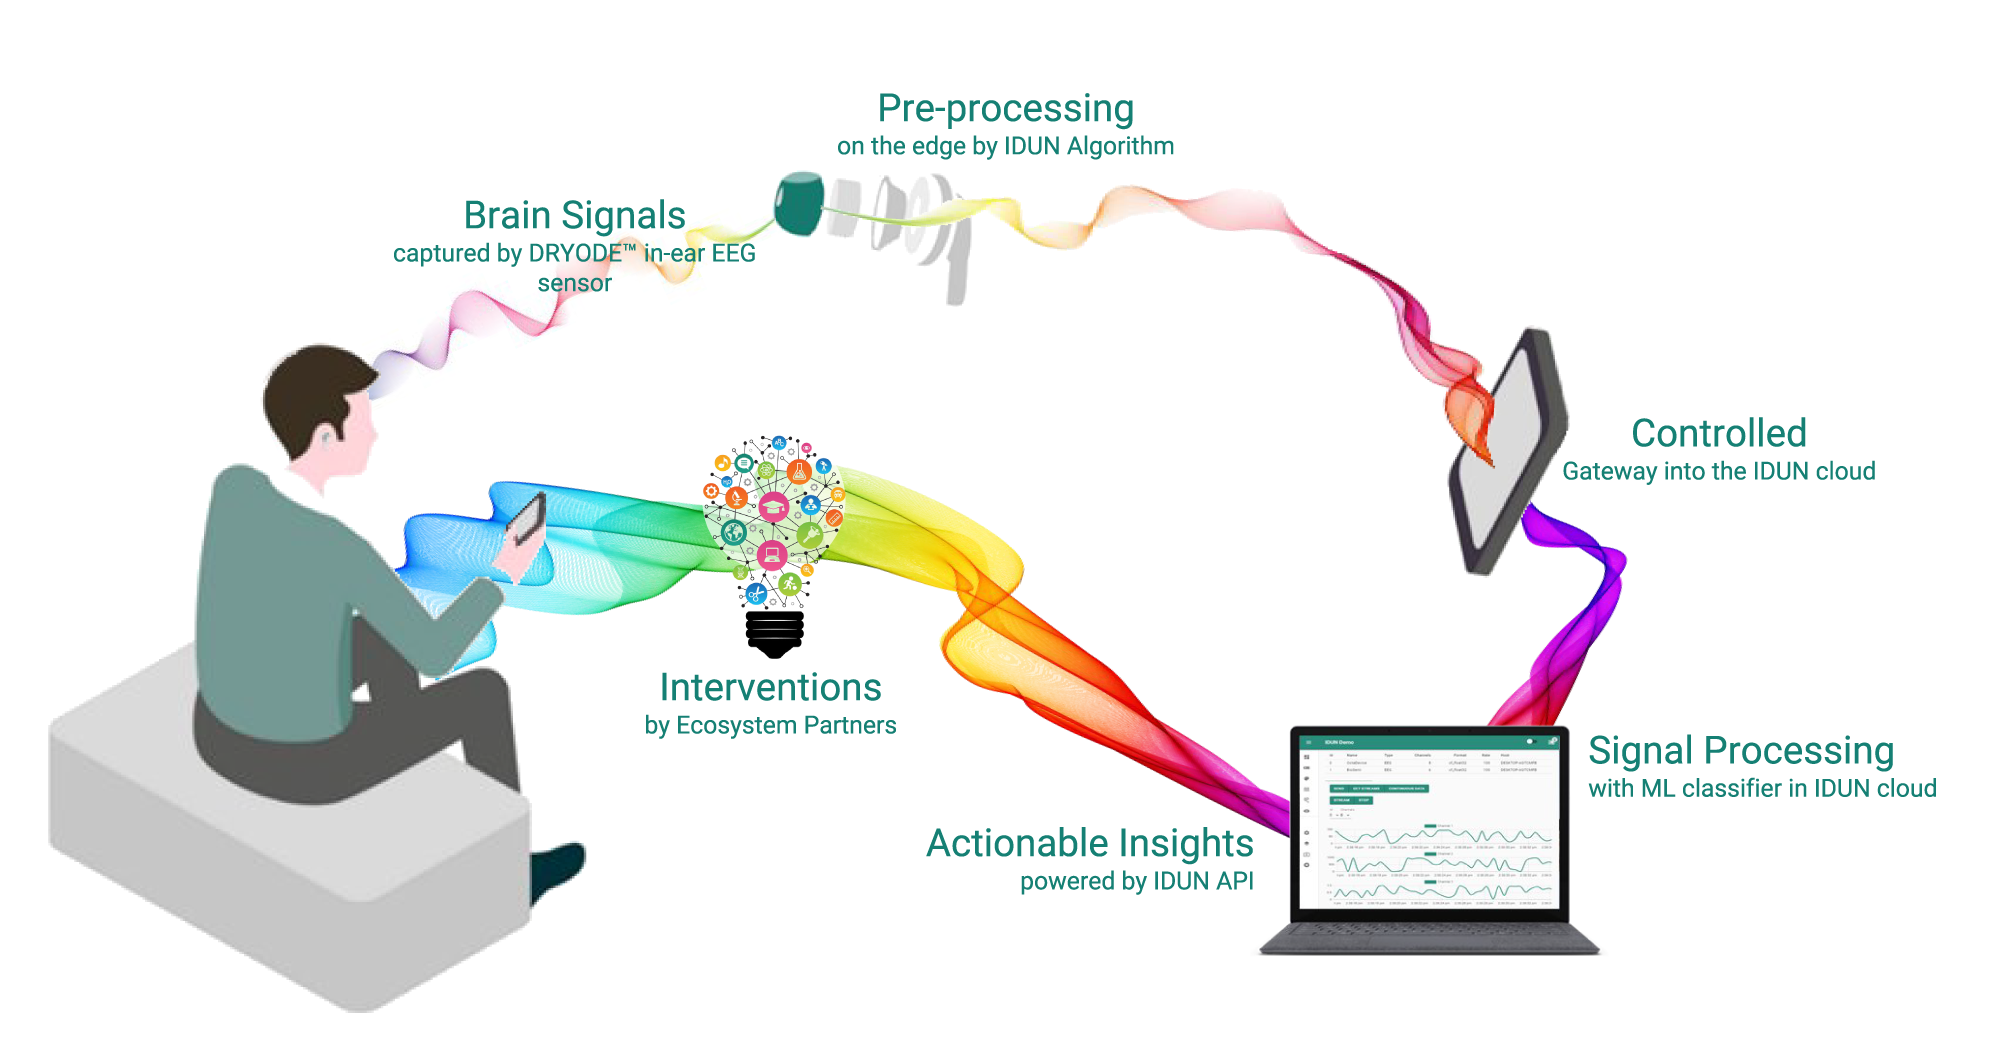
\includegraphics[width=0.75\linewidth]{idun-nip.png}
  \caption{IDUN's vision of a closed neurofeedback loop \citep{idun_guardian_nodate}.}
  \label{fig:idun-nip}
\end{figure}

The mission is essentially that an unobtrusive BCI device, such as an in-ear headset, can be worn for the majority of the day while measuring neural data that is sent in real time to the cloud to process and classify actionable insights that other developers can use to build their interventions (e.g., apps, websites, and games) on top of it to promote mental health and well-being, as described by IDUN in its vision. Furthermore, the aspect of longitudinal data is important, implying that it could be advantageous to store neural data over a long period of time and run classifiers on it from time to time to better understand one's brain.

It is essential to select an appropriate research method in order to develop a system that would fulfil the company's mission and vision. The author chose a case study because it is an effective method for dealing with unusual and atypical cases while also providing new and unexpected perspectives in certain situations.

\section{Procedure}
\label{chapter3-procedure}

This section describes the planned procedure for conducting a case study-based research methodology to develop the proposed software system at IDUN Technologies.

\subsection{Project stages}
\label{chapter3-project-stages}

The goal was to conduct empirical research and examine the use case from various perspectives. In addition, two other methodologies were used in the case study: 1. Expert interviews, which entails locating experts on topics such as cloud or BCI and asking them questions that will assist in answering the research question, and 2. group discussions, which aim at learning about people's attitudes and opinions.

\begin{figure}[!ht]
  \centering
  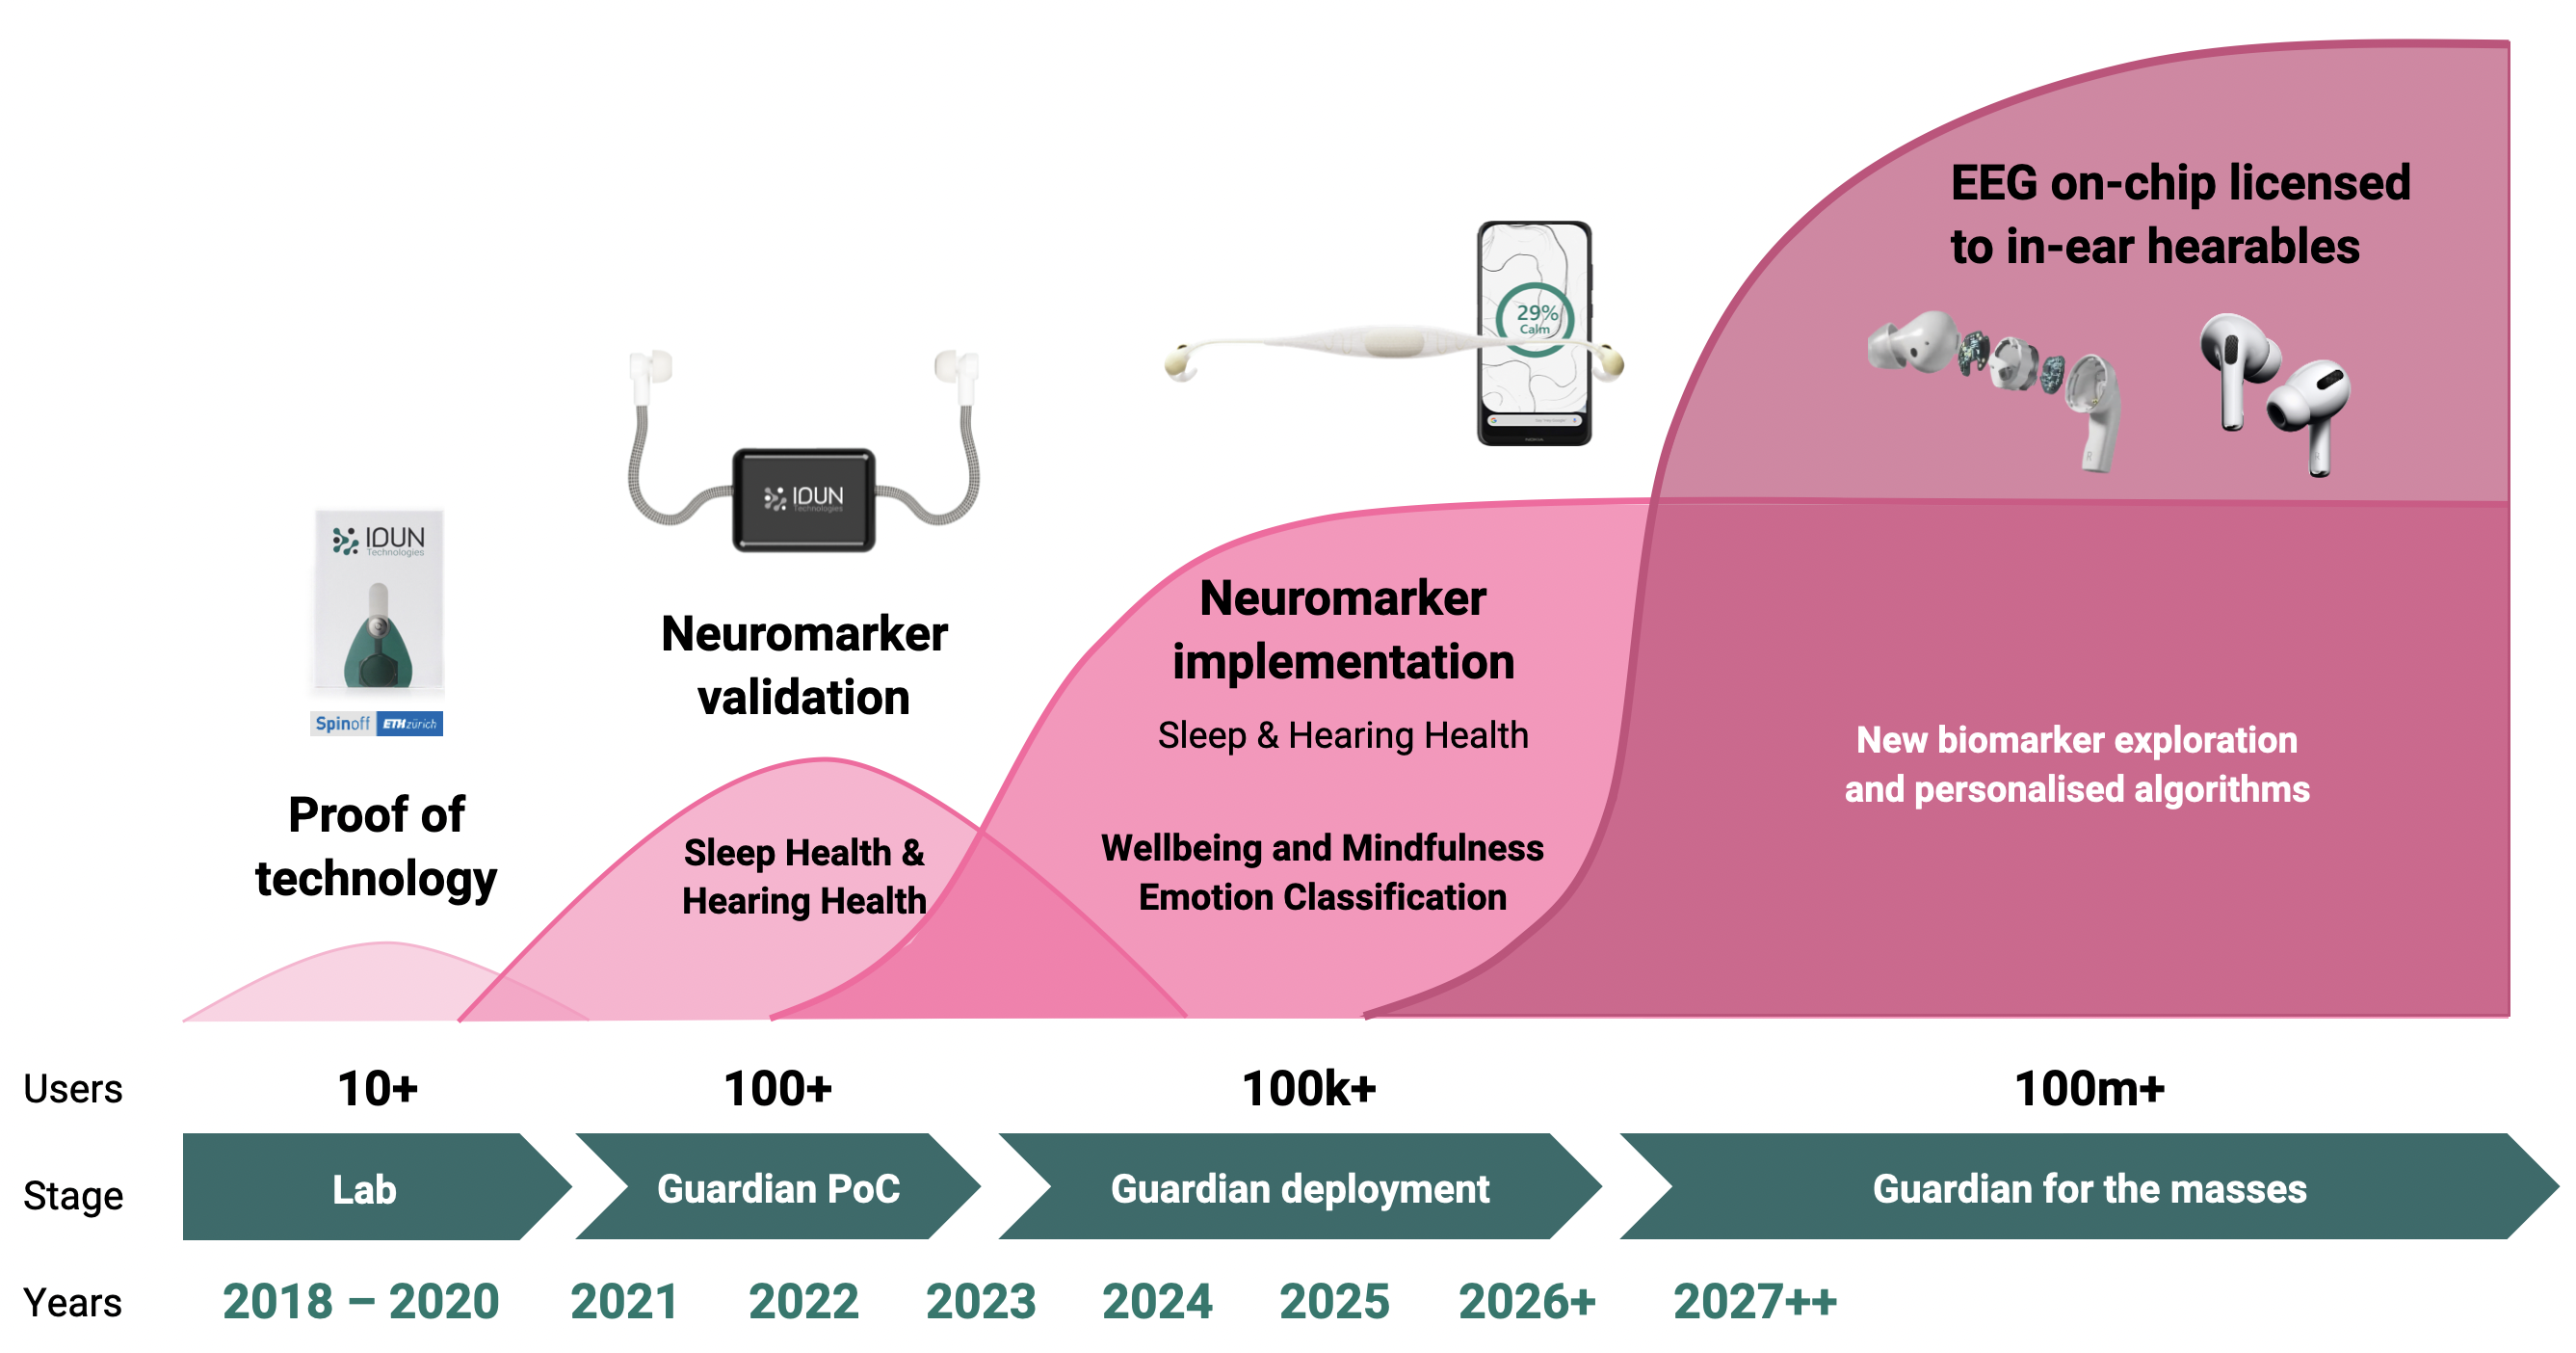
\includegraphics[width=0.75\linewidth]{idun-timeline.png}
  \caption{IDUN's plan to achieve their goals \citep{idun_guardian_nodate}.}
  \label{fig:idun-timeline}
\end{figure}

Before being able to define the project stages it essential to look at the timing of IDUN's roadmap as shown on \autoref{fig:idun-timeline}. There are three important pieces of information: The stage of which the technology resides in, the estimated user base size and the time frames of these stages want to be achieved. The author was working on the version starting to be released in 2023, ergo working on the software system aimed at the Guardian deployment phase. As the company is still in the stage of implementing the first neuromarkers into a real product and is focusing on four use cases due to the size of the company and the mass producibility of hardware and sensors, the sales team is targeting the sale of devices to about 100'000 people.

Another constraint is the deadline of the bachelor's thesis of the author, which is set on the 5th of August 2022. User size, company stages and the deadline for the thesis are important context information for defining the project stages for this use case. Following on \autoref{tab:project-stages} are the proposed project stages to execute the case study:

\begin{table}[!ht]
\centering
\resizebox{\textwidth}{!}{%
\begin{tabular}{
>{\columncolor[HTML]{FFFFFF}}l l}
\cellcolor[HTML]{000000}{\color[HTML]{FFFFFF} Project stage} &
  \cellcolor[HTML]{000000}{\color[HTML]{FFFFFF} Description} \\ \hline
\multicolumn{1}{|l|}{\cellcolor[HTML]{FFFFFF}\textbf{\begin{tabular}[c]{@{}l@{}}1.1 Define key technical\\ requirements and\\ constraints\end{tabular}}} &
  \multicolumn{1}{l|}{\begin{tabular}[c]{@{}l@{}}Based on the internal hardware, the neuroscience and data science departments and the IDUN mission\\ and roadmap, the author needs to define the purely technical requirements and constraints. Some\\ constraints are e.g. hiring of advisors, time limits and risks due to investment rounds. Some purely\\ technical requirements come from e.g. the firmware team or the material scientists, such as maximum\\ latency or the data structure of the digitalised EEG.\end{tabular}} \\ \hline
\multicolumn{1}{|l|}{\cellcolor[HTML]{FFFFFF}\textbf{\begin{tabular}[c]{@{}l@{}}1.2 Extensive literature\\ research\end{tabular}}} &
  \multicolumn{1}{l|}{\begin{tabular}[c]{@{}l@{}}Already since the beginning of the original bachelor thesis, the author started to do literature research in\\ the field of BCI, which is very helpful for the new focus. Further literature review now includes books\\ on data intensive applications and cloud, articles and research papers.\end{tabular}} \\ \hline
\multicolumn{1}{|l|}{\cellcolor[HTML]{FFFFFF}\textbf{\begin{tabular}[c]{@{}l@{}}2.1 External user\\ interviews\end{tabular}}} &
  \multicolumn{1}{l|}{\begin{tabular}[c]{@{}l@{}}Defining users personas with IDUN's product manager, application engineer and sales team, finding\\ real people to represent these personas, preparing an external interview framework and questions,\\ gathering as many insights as possible.\end{tabular}} \\ \hline
\multicolumn{1}{|l|}{\cellcolor[HTML]{FFFFFF}\textbf{\begin{tabular}[c]{@{}l@{}}2.2 Creative workshop and\\ prototyping\end{tabular}}} &
  \multicolumn{1}{l|}{\begin{tabular}[c]{@{}l@{}}Based on the insights from the customer interviews, conduct a creative workshop with IDUN's product\\ manager and application engineer. The results are design artefacts such as wireframes, user flows,\\ interactive prototypes and architecture diagrams.\end{tabular}} \\ \hline
\multicolumn{1}{|l|}{\cellcolor[HTML]{FFFFFF}\textbf{\begin{tabular}[c]{@{}l@{}}3.1 Internal group\\ discussions\end{tabular}}} &
  \multicolumn{1}{l|}{\begin{tabular}[c]{@{}l@{}}The design artefacts are used for an internal validation with the department heads. Several group\\ discussions are held with each department, ranging from materials science to business development.\\ Based on the group discussions, the artefacts are adapted and improved.\end{tabular}} \\ \hline
\multicolumn{1}{|l|}{\cellcolor[HTML]{FFFFFF}\textbf{3.2 Expert interviews}} &
  \multicolumn{1}{l|}{\begin{tabular}[c]{@{}l@{}}Define experts in different areas of BCI, cloud and EEG, and neuroethics. Create a framework for\\ expert interviews and questions that are still unclear or open based on the design artefacts. Conduct\\ expert interviews and gather as many insights as possible to adapt and improve the design artefacts.\end{tabular}} \\ \hline
\multicolumn{1}{|l|}{\cellcolor[HTML]{FFFFFF}\textbf{4. Start bootstrapping}} &
  \multicolumn{1}{l|}{\begin{tabular}[c]{@{}l@{}}While the design process is still ongoing, you can already start implementing the most important\\ technical requirements, with anything that is a flexible bootstrapping of internal development\\ processes to ensure quality assurance, for example, not being tied to the other phases.\end{tabular}} \\ \hline
\multicolumn{1}{|l|}{\cellcolor[HTML]{FFFFFF}\textbf{\begin{tabular}[c]{@{}l@{}}5. Iterative and agile\\ implementation via\\ Scrum\end{tabular}}} &
  \multicolumn{1}{l|}{\begin{tabular}[c]{@{}l@{}}IDUN works with Scrum, for this the author has introduced Scrum in the research and development\\ department. Scrum at IDUN has three-week sprints and there are ten sprints from January 2022 to the\\ end of July 2022 that can be used to go through the design process and implement the designs. In the\\ process, there are several iterative processes to validate and test the increments of the system based on\\ insights from the implementation, ongoing literature research, insights from other departments or the\\ design process that is still ongoing.\end{tabular}} \\ \hline
\end{tabular}%
}
\vspace{10pt}
\caption{Project stages to answer the research question of this thesis.}
\vspace{-5pt}
\label{tab:project-stages}
\end{table}

Number 1.1 is crucial before starting anything else. Number 1.2 is always in progress. Numbers 2.1 to 3.2 take place simultaneously while number 4 is in progress. As soon as number 3.2 and 4. are completed, number 5. can be started.

% - Identify problems with current system
% - Identify and reason about key technical requirements that go well with IDUN's mission and vision
% - Extensive literature research on other BCI systems through the cloud which was already going on due to original bsc project
% - Identify personas for upcoming release
% - Find people representing the personas
% - Interview and consolidate insights from real people
% - Creative workshop based on insights (show image)
% - Design artefacts: SDK, Console Web App
% - Ethics Workshop
% - Validate with internal tech requirements from other departments
% - Define requirements based on design artefacts
% - Find relevant experts in related fields
% - Expert discussions based on requirements and design artefacts
% - Already implementing the key technical requirements (bootstrapping for avoiding things such as with the previous system)
% - Validate technicalities with key technical requirements such as performance and quality
% - Create demo applications with as soon as existing software to test

\subsection{Group discussions}
\label{chapter3-group-discussions}

\subsection{Expert interviews}
\label{chapter3-expert-interviews}

\section{Outcomes}
\label{chapter3-outcomes}

% non-trivial, n-body system, Services, batch processing and near real time streaming, shared nothing, encrypted, total order broadcast etc. => all insights that were gained for the N/CI and the task to define a N/CI on its own as well + Systems of record and derived data system (p 602 to cite) ==> add some parts to the implementation chapter

% However, in practice, it appears that simply making data available quickly—even if it is in a quirky, difficult-to-use, raw format—is often more valuable than trying to decide on the ideal data model up front [54].

\section{Reflection}
\label{chapter3-reflection}

\section{Further development}
\label{chapter3-further-development}

% - Distributed system, data warehouse and other constraints that came up during the research etc. + non-critical, no-real-time needed, system on a chip is coming and what will it bring for things, or going directly via the internet and not the device itself, why not making that decision
% - Data warehouse difference between data lake
% - feature store

% - First, they were randomly assigned to treatment and placebo group
% - Both groups: 60 minutes intervention
% - Treatment group: first,… next,…
% - Placebo group: first, …next,…
% - Finally, they filled out the depression questionnaire
% o Did you describe everything that is needed to replicate your research?
% o Did you cite the sources of your methods or paradigms?

\nomenclature[nip]{NIP}{Neuro-Intelligence Platform}
\nomenclature[spa]{SPA}{Single-page application}
\nomenclature[gdk]{GDK}{Guardian Development Kit}
\nomenclature[mqtt]{MQTT}{IBM MQ Telemetry Transport}
